\chapter{The Quantum Theory of Light}
\section{Heartz's Experiments; Light as EM Wave}
    
    \paragraph{$\bullet$} Between 1865 and 1873, James Clerk Maxwell, and according to his theory, 
    an alternating current would set up fluctuating electric and magnetic fields in the 
    region surrounding the original disturbance.
    \paragraph{$\bullet$} These waves were predicted to have a frequency equal to the frequency of the current oscillations.
    \paragraph{$\bullet$} And more importnatly, they would behave in every way like \textit{light}.
    \paragraph{$\bullet$} Naturally this led to the unifying and simplifying postulate that light was also a 
    type of Maxwell wave or electromagnetic disturbance, created by extremely high frequency electric oscillators in matter.
    \paragraph{$\bullet$} it was apparent that this model of light emission was incapable of direct experimental 
    verification, because the highest electrical frequencies then attainable were about $10^9Hz$.

    \begin{wrapfigure}{r}{0.25\linewidth}
        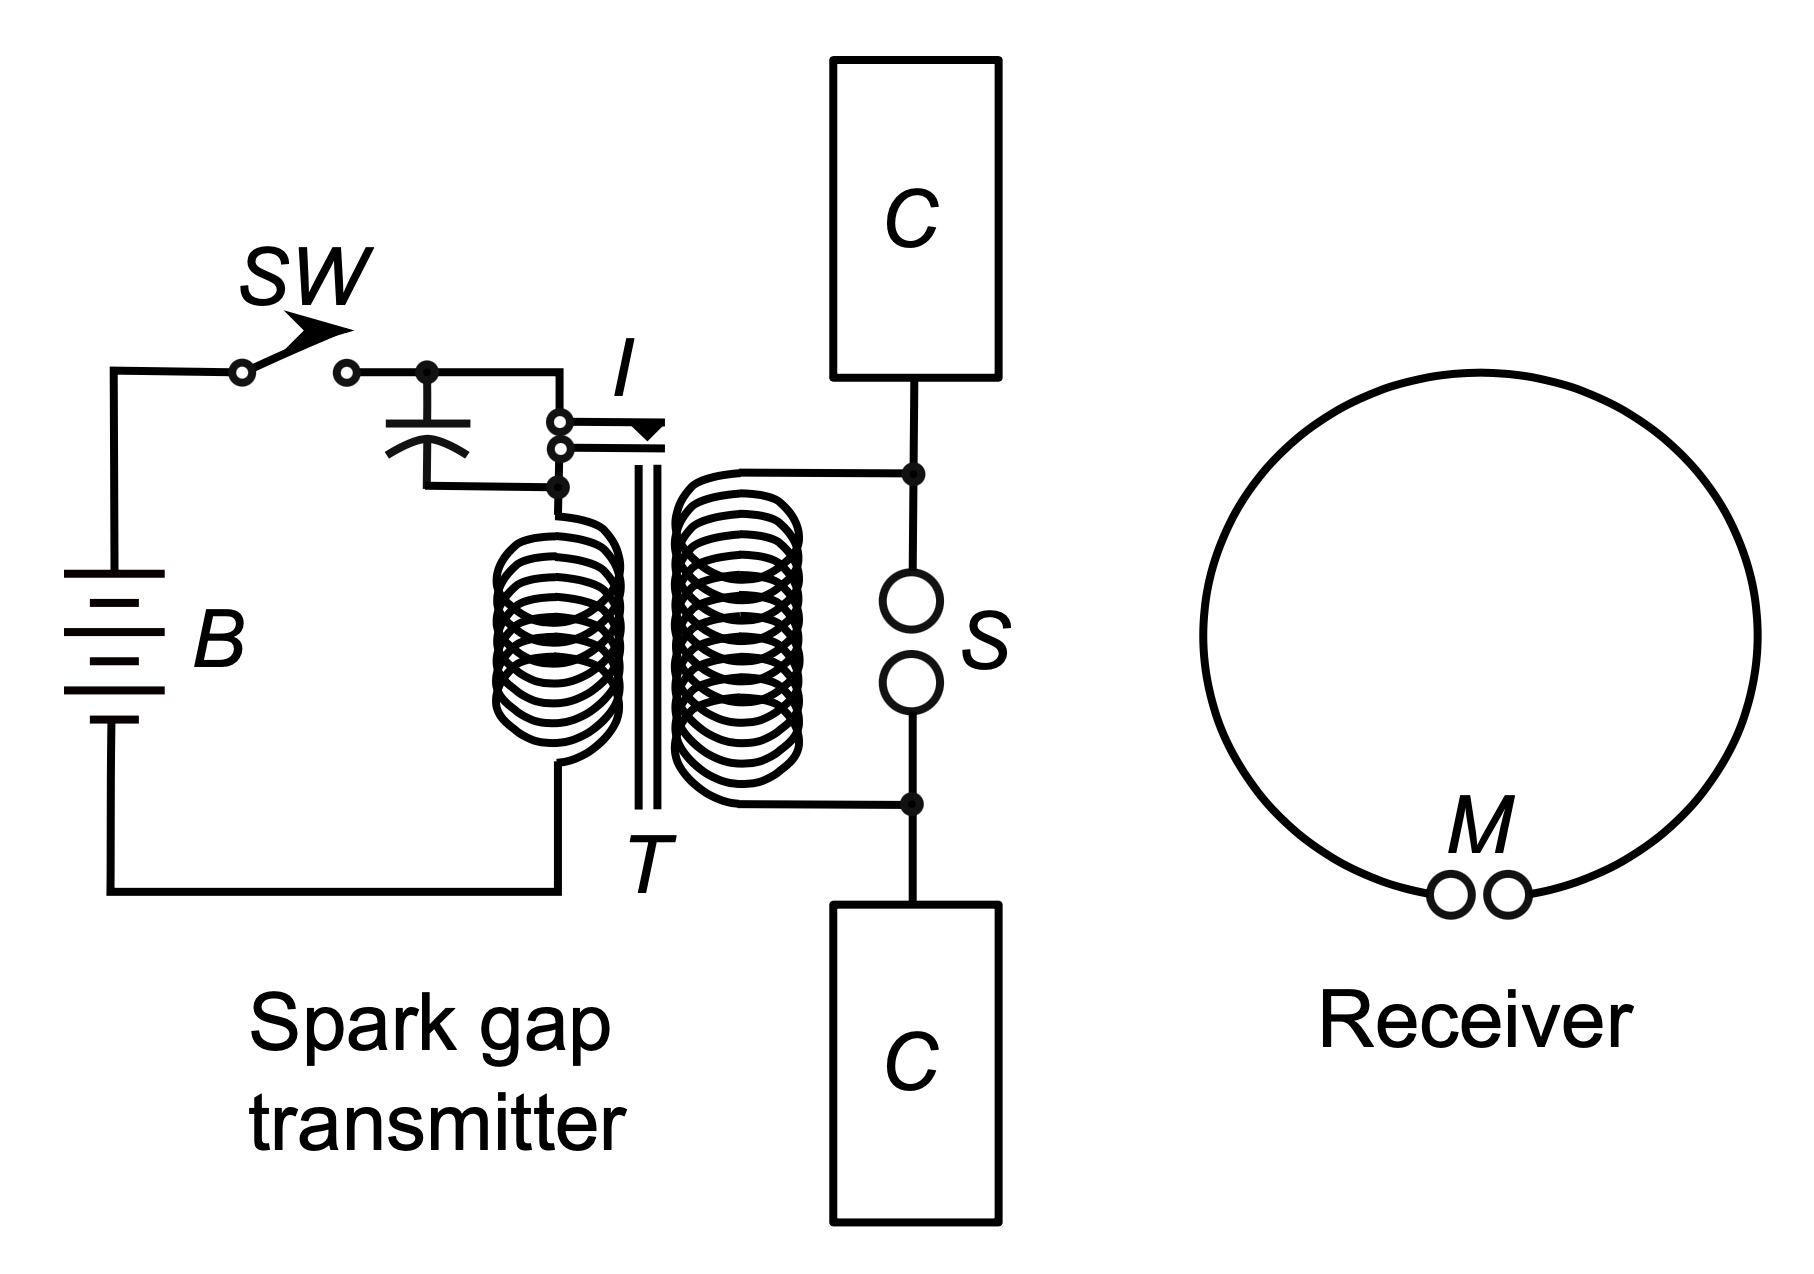
\includegraphics[width=0.9\linewidth]{figures/Hertz_transmitter.png}
        \caption{Heartz's Transmitter.}
        \label{fig:heartz's transmitter}
    \end{wrapfigure}

    \paragraph{$\bullet$} Heinrich Hertz showed that Maxwell’s theory was correct and that an oscillating electric 
    current does indeed radiate electromagnetic waves that possess every characteristic of light 
    except the same wavelength as light.  

    \paragraph{$\bullet$} By using a simple spark gap oscillator in Fig.\eqref{fig:heartz's transmitter}.

    \paragraph{$\bullet$} Hertz next proceeded to show that these electromagnetic waves could be reflected, 
    refracted, focused, polarized, and made to interfere—- in short, he convinced physicists 
    of the period that Hertzian waves and light waves were one and the same.
    
\section{Blackbody Radiation}
    The problem is to predict the radiation intensity at a given wavelength emitted by 
    a hot glowing solid at a specific temperature.
    \paragraph{$\bullet$} In 1792, Thomas Wedgwood observed that all the objects in his ovens, regard- less 
    of their chemical nature, size, or shape, became red at the same tempera- ture.
    \paragraph{$\bullet$} In 1859, Gustav Kirchhoff proved a theorem when he showed by arguments based 
    on thermodynamics that for any body in thermal equilibrium with radiation the emitted power is 
    proportional to the power absorbed. More specifically,
    \coloredeq{Kirchhoff emitted power theorem}{e_f=J(f, T)A_f}
    {\tiny \begin{itemize}
        \item $e_f$ is the power emitted per unit area per unit frequenct by a heated object.
        \item $A_f$ is the absorption power (fraction of the incident power absorbed per 
        unit area per unit frequency by the heated object).
        \item $J(f, T)$ is a universal function (the same for all bodies) that depends only on $f$.
    \end{itemize}}

    \paragraph{$\bullet$} A \textbf{blackbody} is defined as an object that absorbs all the electromagnetic 
    radiation falling on it and consequently appears black. It has $a_f=1$ for all frequencies 
    and so Kirchhoff’s theorem for a blackbody becomes,
    \begin{align} \label{kirchhoff theorm blackbody}
        e_f=J(f, T)
    \end{align}

    \paragraph{$\bullet$} Eq.\eqref{Kirchhoff emitted power theorem} shows that the power emitted only
    per unit area per unit frequency by a blackbody depends only on the light frequency and the 
    temperature.

    \paragraph{$\bullet$} Because absorption and emission are connected by Kirchhoff’s theorem, 
    we see that a \textit{blackbody} or perfect absorber is also an ideal \textit{radiator}.\\
    In practice, a small opening in any heated \textit{cavity}, such as a port in an oven, behaves 
    like a blackbody because such an opening traps all incident radiation.

    \paragraph{$\bullet$} In 1879, Josef Stefan found experimentally that the total power per unit 
    area emitted at all frequencies by a hot solid, was proportional to the fourth 
    power of its absolute temperature. Therefore, \textit{Stefan’s law} may be written as
    \coloredeq{eq:stefan's law}{e_{total}=\int_0^\infty e_f \, df = \sigma T^4}
    {\tiny \begin{itemize}
        \item $e_{total}$ is the power per unit area emitted at the surface of the blackbody at all frequencies.
        \item $e_f$ is the power per unit area per unit frequency emitted by the blackbody.
        \item $T$ is the absolute temperature of the body.
        \item $\sigma$ is the Stefan – Boltzmann constant $\sigma= \SI[per-mode=symbol]{3e5}{\W\per\m\squared\per\K\tothe{4}}$.
    \end{itemize}}
    A body that is not an ideal radiator will obey the same general law but with a 
    coefficient, $a$, less than 1: \begin{align}\label{emitted power from non-ideal body}e_{total}=a \sigma T^4\end{align}

    \begin{wrapfigure}{r}{0.25\linewidth}
        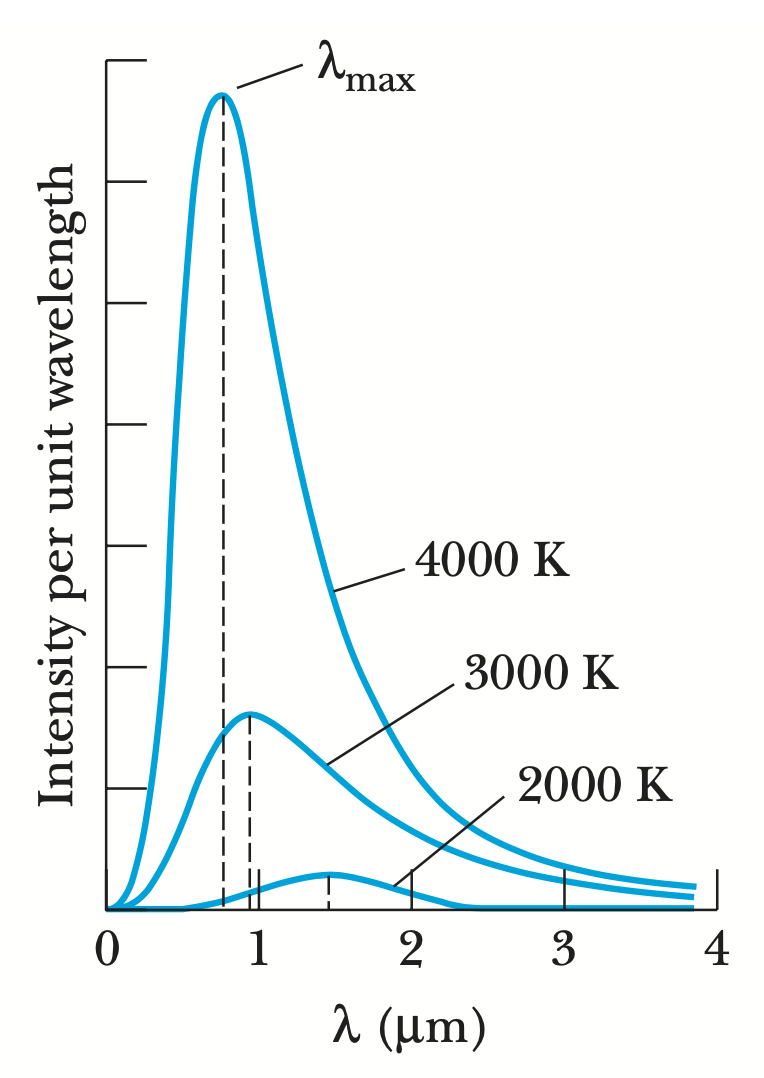
\includegraphics[width=0.9\linewidth]{figures/blackbody emission.png}
        \caption{Emission from a glowing solid.}
        \label{fig:blackbody emission}
    \end{wrapfigure}
    
    \paragraph{$\bullet$} Notice that in Fig.\eqref{fig:blackbody emission} $\lambda_{max}$ shifts
    to shorter wavelengths as the blackbody gets hotter.\\
    In 1893, Wilhelm Wien proposed a general form for the blackbody distribution law 
    $J(f, T)$ that gave the correct experimental behavior of $\lambda_{max}$ with temperature. This 
    law is called \textbf{Wien’s displacement law} and may be written
    \begin{align} \label{Wien's displacement law}
        \lambda_{max} T = \SI{2.898e-3}{\m\K}
    \end{align}
    {\tiny \begin{itemize}
        \item $\lambda_{max}$ is the the blackbody’s maximum intensity.
        \item $T$ is the absolute temperature of the surface.
    \end{itemize}}
    
    \paragraph{$\bullet$} Let's consider the energy per unit volume per unit frequency of 
    the radiation within the blackbody cavity, $u( f, T )$. For light in equilibrium with 
    the walls, the power emitted per square centimeter of opening is simply proportional to 
    the energy density of the light in the cavity.

    \paragraph{$\bullet$} An important guess as to the form of the universal function $u(f, T)$ was
    made in 1893 by Wien and had the form 
    \begin{align} \label{Wien's exponential law}
        u(f,T) = A f^3 e^{- \beta f/T}
    \end{align}
    {\tiny \begin{itemize}
        \item $A$ and $\beta$ are constants
    \end{itemize}}

    \paragraph{$\bullet$} Within a year Friedrich Paschen, had confirmed Wien’s guess 
    by working in the then difficult infrared range of 1 to \SI{4}{\mu\m} and at temperatures 
    of 400 to \SI{1600}{\K}.Paschen had made most of his 
    measurements in the maximum energy region of a body heated to 1500K and had found good 
    agreement with Wien’s exponential law. In 1900, however, Lummer and Pringsheim extended 
    the measurements to \SI{18}{\mu\m}, and Rubens and Kurlbaum went even farther$-$ to \SI{60}{\mu\m}.
    Both teams concluded that Wien’s law failed in this region.

    \paragraph{\color{c3}Enter Planck}
    On a Sunday evening early in October of 1900, Max Planck discovered the famous blackbody formula.

    Planck knew that Wien’s law agreed well with the data at high frequency and indeed had been 
    working hard for several years to derive Wien’s exponential law from the principles of statistical 
    mechanics and Maxwell’s laws. See Eq.\eqref{eq:Plank distribution law}
    

    \paragraph{\color{c3}The Quantum Energy}
    Planck was convinced that blackbody radiation was produced by vibrating submicroscopic 
    electric charges, which he called \textit{resonators}. He assumed that the walls of a glowing 
    cavity were composed of literally billions of these \textit{resonators} (whose exact nature was 
    unknown at the time), all vibrating at different frequencies. Hence, according to Maxwell, 
    each \textit{oscillator} should emit radiation with a frequency corresponding to its vibration 
    frequency. \textbf{Also according to \textit{classical Maxwellian theory}, an oscillator of frequency $f$ 
    could have \textbf{any} value of energy and could change its amplitude continuously as it 
    radiated any fraction of its energy.}

    \paragraph{$\bullet$} This is where Planck made his revolutionary proposal. 
    To secure agreement with experiment, Planck had to assume that the total energy of a 
    resonator with mechanical frequency $f$ could only be an integral multiple of $hf$ or
    \coloredeq{eq:Planck resonator energy}{E_{resonator}=nhf\quad n=1, 2, 3, \dots}
    he concluded that emission of radiation of frequency f occurred when a resonator dropped 
    to the next lowest energy state.\\
    Thus the resonator can change its energy only by the difference $\Delta{E}$ according to
    \begin{align} \label{eq:energy change of hf}
        \Delta{E} = hf
    \end{align}
    \textit{That is, it cannot lose just any amount of its total energy, but only a finite amount, $hf$, 
    the so-called \textbf{quantum} of energy.}
    
    \paragraph{$\bullet$} Planck explained the continuous spectrum of the blackbody by assuming 
    that \textit{the heated walls contained resonators vibrating at many different frequencies}, each 
    emitting light at the same frequency as its vibration frequency.

    \paragraph{$\bullet$}  considering the conditions leading to equilibrium between the \textit{wall resonators}
    and the \textit{radiation} in the blackbody cavity, he found that the 
    spectral energy density $u(f, T)$ could be expressed as
    \coloredeq{eq:spectral energy desity}{u(f, T)\, df= \bar{E}N(f)\, df}
    {\tiny \begin{itemize}
        \item $N(f)$ number of oscillators having frequency between $f$ and $f + df$.
        \item $\bar{E}$ average energy emitted per oscillator.
    \end{itemize}}

    Furthermore, Planck showed that the number of oscillators with frequency
    between $f$ and $f + df$ was proportional to $f^2$ or 
    \begin{align}
        \label{eq:number of oscillator}
        N(f)\, df = \frac{8 \pi f^2}{c^3} \, df
    \end{align}

\section{The Rayleigh-Jeans Law and Planck's Law}
    Both Planck’s law and the Rayleigh–Jeans law\footnote{the classical theory of blackbody radiation formulated by 
    Lord Rayleigh, John William Strutt, 1842–1919, English physicist, and James Jeans, 1887–1946, English 
    astronomer and physicist} may be derived using the idea that the blackbody radiation energy per unit volume can expressed
    as in Eq.\eqref{eq:spectral energy desity}. We will consider \textbf{Rayleigh–Jeans} and \textbf{Planck} calculations 
    to see the effect on $u(f, T)$ of calculating $\bar{E}$ from a \textit{continuous} distribution of classical oscillator energies 
    (Rayleigh–Jeans) as opposed to a \textit{discrete} set of quantum oscillator energies (Planck).

    \paragraph{\color{c3}Rayleigh-Jeans Law} % (fold)
    \label{par:Rayleigh-Jeans Law}     
    \begin{wrapfigure}{r}{0.2\linewidth}
        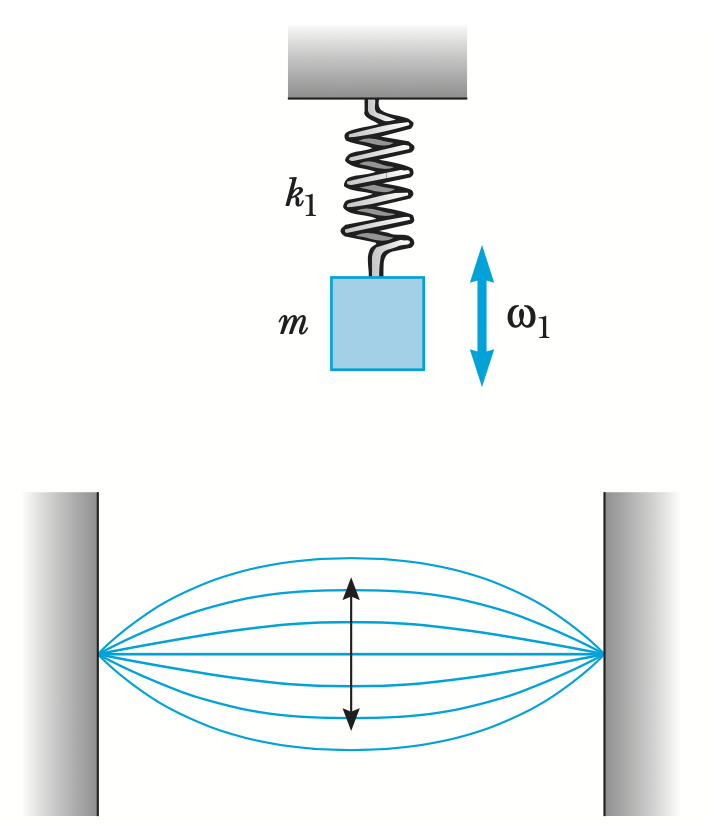
\includegraphics[width=0.9\linewidth]{figures/standing wave.png}
        \caption{A one-dimensional harmonic oscillator.}
        \label{fig:A one-dimensional harmonic oscillator}
        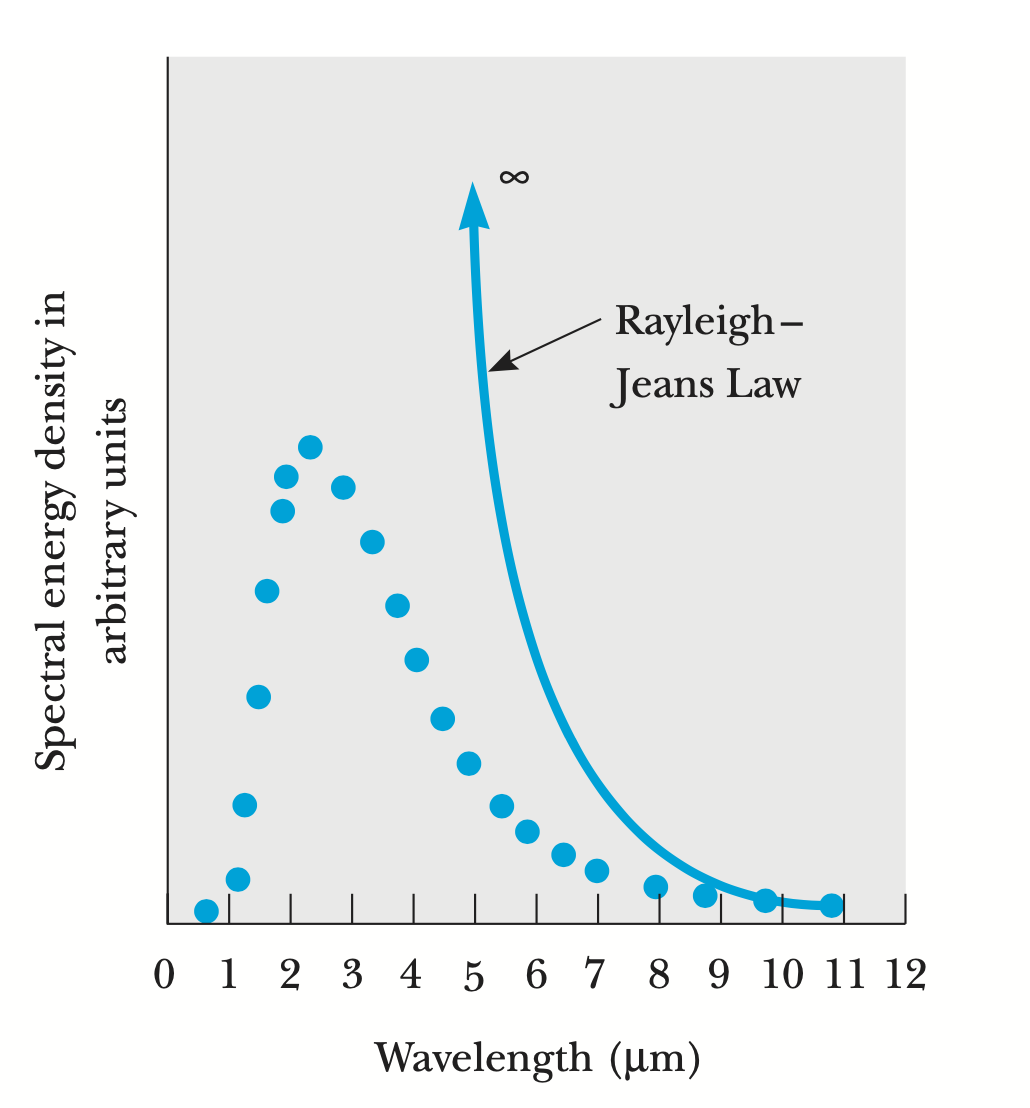
\includegraphics[width=0.9\linewidth]{figures/spectral energy density.png}
        \caption{The failure of the classical Rayleigh–Jeans law Eq.\eqref{eq:Rayleigh-Jeans energy density} 
        to fit the observed spectrum of a blackbody heated to 1000 K.}
        \label{fig:spectral energy density}
    \end{wrapfigure}   

    \textit{While Planck concentrated on the thermal equilibrium of cavity radiation with oscillating electric charges in 
    the cavity walls, Rayleigh concentrated directly on the electromagnetic waves in the cavity}. 
    \paragraph{\color{c3}$\bullet$}Rayleigh and Jeans 
    reasoned that the \textit{standing electromagnetic waves} in the cavity could be considered to have a \texttt{temperature} $T$, 
    because they constantly exchanged energy with the walls and caused a thermometer within the cavity to reach 
    the same temperature as the walls. Further, they considered a \textit{standing polarized electromagnetic wave} to be 
    equivalent to a one-dimensional oscillator \eqref{fig:A one-dimensional harmonic oscillator}. 

    \paragraph{\color{c3}$\bullet$}Using the same general idea as Planck, they expressed 
    the energy density as a product of the number of standing waves (oscillators) and the average energy per 
    oscillator. They found the average oscillator energy $\bar{E}$ to be independent of frequency and equal to $k_B T$ from 
    the \textit{Maxwell-Boltzmann distribution law} (see Chapter 10). According to this distribution law, 
    \begin{align}
        \label{eq:probability of finding a system}
        P(E) = P_0\, e^{-(E-E_0)/k_B T}
    \end{align}
    {\tiny \begin{itemize}
        \item the probability $P$ of finding an individual system (such as a molecule or an atomic oscillator) 
        \item with energy $E$ above some  
        \item minimum energy($E_0$) in a large group of systems at 
        \item temperature $T$
        \item where P0 is the probability that a system has the minimum energy.
    \end{itemize}}
    
    \paragraph{\color{c3}$\bullet$} In the case of a discrete set of allowed energies, the average energy($\bar{E}$) is given by
    \begin{align}
        \label{eq:average energy}
        \bar{E} = \frac{\Sigma E\, P(E)}{\Sigma P(E)}
    \end{align}
    where division by the sum in the denominator serves to normalize the total probability to 1.

    \paragraph{\color{c3}$\bullet$} \textit{In the classical case considered by Rayleigh}, an oscillator can have any energy $E$ in
    a continuous range from 0 to $\infty$. Thus the Eq.\eqref{eq:average energy} muse be replaced with integrals, so 
    \begin{align}
        \label{eq:average energy integral}
        \bar{E} = \frac{\int_0^\infty Ee^{-E/k_B T}\, dE}{\int_0^\infty e^{-E/k_B T}\, dE} = k_B T
    \end{align}
    The derivation of the density of modes, $N( f )\, df$, gives
    \begin{align}
        \label{eq:density of modes}
        N(f)\, df = \frac{8 \pi f^3}{c^3} \, df \qquad \text{or in wavelength} \qquad 
        N(\lambda) \, d\lambda = \frac{8 \pi }{\lambda^4}\, d\lambda  
    \end{align}
    The spectral energy density is simply the \textit{density of modes} multiplied by $k_B T$, or
    \begin{align}
        \label{eq:Rayleigh-Jeans energy density}
        u(f, T)\, df = \frac{8 \pi f^2}{c^3} k_B T\, df \qquad \text{or in wavelength} \qquad 
        u(\lambda, T)\, d\lambda = \frac{8 \pi}{\lambda^4} k_B T\, d\lambda
    \end{align}
    
    \paragraph{\color{c3}$\bullet$} However, as in Figure~\ref{fig:spectral energy density}, this classical expression, 
    known as the \textit{Rayleigh–Jeans law}, does not agree with the experimental results in the short wavelength region.
    Eq.\eqref{eq:Rayleigh-Jeans energy density} diverges as $\lambda \to 0$, predicting unlimited energy emission in the 
    ultraviolet region, which was dubbed the “ultraviolet catastrophe”. To conclude that the classical theory fails 
    to explain blackbody radiation.
    % paragraph Rayleigh-Jeans Law (end)

    \paragraph{\color{c3}Planck Law} % (fold)
    \label{par:Planck Law}
    Planck concentrated on the energy \textit{states of resonators} in the cavity walls and used the condition that the 
    \texttt{resonators and cavity radiation were inequilibrium} to determine the spectral quality of the radiation. 
    By thermodynamic reasoning (and apparently unaware of Rayleigh’s derivation), he arrived at the same expression 
    for $N( f )$ as Rayleigh. However, Planck arrived at a different form for $E$ by allowing only \textit{discrete} values of 
    energy for his resonators. He found, using the Maxwell-Boltzmann distribution law,
    \begin{align}
        \label{eq:plank average energy}
        \bar{E} = \frac{hf}{e^{hf/k_b T}-1}
    \end{align}
    Multiplying $\bar{E}$ by $N(f)$ gives the Planck distribution law,
    \coloredeq{eq:Plank distribution law}{
        \begin{aligned}
            u(f, T)\, df &= \frac{8\pi f^2}{c^3} \left(\frac{hf}{e^{hf/k_B T}-1}\right)\, df \\
            \text{or in wavelength} \qquad \qquad 
            u(\lambda, T)\, d\lambda &= \frac{8\pi h c}{\lambda^5(e^{hc/\lambda k_B T}-1)}\, d\lambda
        \end{aligned}
    }
    {\tiny \begin{itemize}
        \item $h$ Planck's constant \SI{6.626e-34}{\J\s}
        \item $k_B$ Boltzmann's constant \SI{1.380e-23}{\J\per\K}
    \end{itemize}}
    \noindent
    In summary, Planck arrived at his blackbody formula by making two startling assumptions: 
    \begin{enumerate}
        \item The energy of a charged oscillator of frequency $f$ is limited to discrete values $nhf$.
        \item During emission or absorption of light, the change in energy of an oscillator is $hf$.
    \end{enumerate}
    
    \paragraph{\color{c3}$\bigstar$} By integrating Eq.\eqref{eq:Plank distribution law} for $0 \to \infty$ we will get 
    Stefan’s law in Eq.\eqref{eq:stefan's law}.
    % paragraph Planck Law (end)

\section{Light Quantization and The Photoelectric Effect}
    Einstein recognized an inconsistency between Planck’s quantization of oscillators in the walls 
    of the blackbody and Planck’s insistence that the cavity radiation consisted of classical electromagnetic waves.

    \paragraph{\color{c3}$\bigstar$} By showing that the change in entropy of blackbody radiation was like 
    the change in entropy of an ideal gas consisting of independent particles, Einstein reached the conclusion 
    that light itself is composed of “grains,” irreducible finite amounts, or quanta of energy.

    \begin{wrapfigure}{r}{0.2\linewidth}
        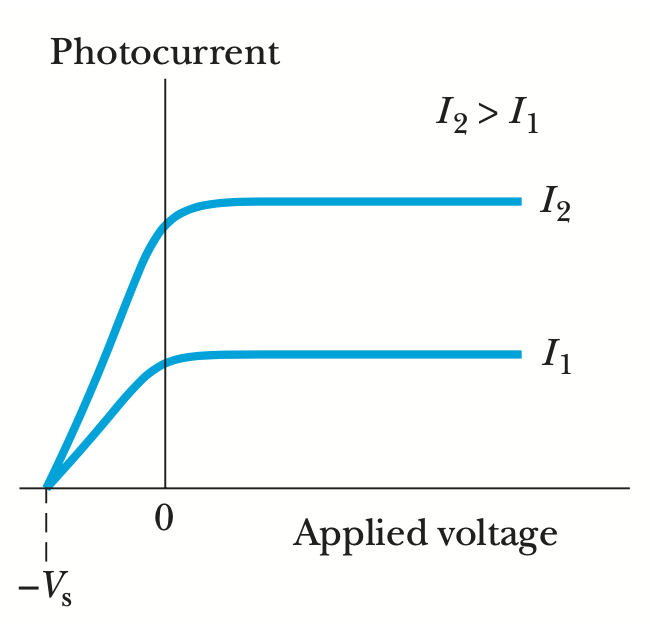
\includegraphics[width=0.9\linewidth]{figures/photocurrent versus applied voltage.png}
        \caption{Photocurrent versus applied voltage}
        \label{fig:Photocurrent versus applied voltage}
        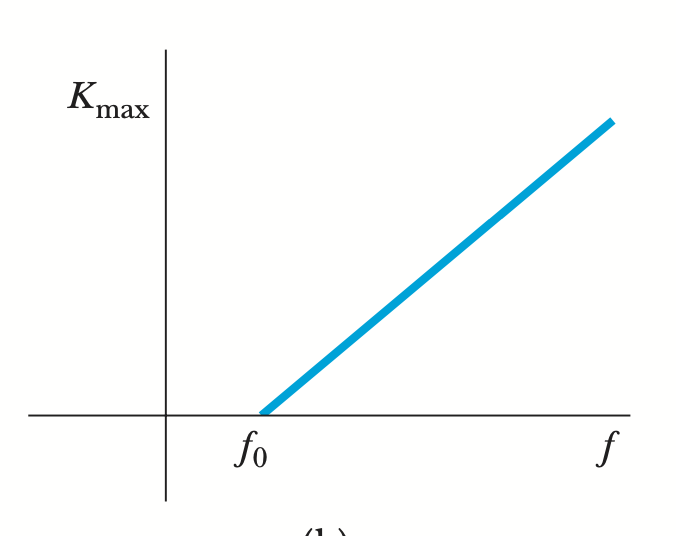
\includegraphics[width=0.9\linewidth]{figures/Kmax.png}
        \caption{$K_{max}$ versus frequency}
        \label{fig:Kmax versus frequency}
    \end{wrapfigure}

    \paragraph{$\bullet$} Hertz first established that clean metal surfaces emit charges when exposed to 
    ultraviolet light. In 1888 Hallwachs discovered that the emitted charges were negative, 
    and in 1899 J. J. Thomson showed that the emitted charges were electrons, now called photoelectrons.

    \paragraph{$\bullet$} In 1902,  Philip Lenard was studying the photoelectric effect with 
    intense carbon arc light sources. He found that electrons are emitted from the metal with a range of 
    velocities and that the maximum kinetic energy of photoelectrons, $K_{max}$, does not depend on the 
    \textit{intensity} of the exciting light. He lso indicated that $K_{max}$ increases with light \textit{frequency}.

    \paragraph{$\bullet$} In the photoelectric setup, $K_{max}$ is easily measured by applying a retarding voltage and gradually 
    increasing it until the most energetic electrons are stopped and the photocurrent becomes zero. At this point,
    \begin{align}
        \label{eq:Kmax of a photoelectron}
        K_{max} = \frac{1}{2} m_e v^2_{max} = eV_s
    \end{align}
    
    As shown in Fig.\eqref{fig:Photocurrent versus applied voltage} Lenard found that 
    $K_{max}$ or $V_s$ is independent of light intensity $I$.\\
    The classical electromagnetic theory has major difficulties explaining:
    \begin{enumerate}
        \item The linear dependence of  $K_{max}$ on light frequency, shown in Fig.\eqref{fig:Kmax versus frequency}.
        \item There is no \textit{time lag} between the start of illumination and the start of the photocurrent.
    \end{enumerate}

    \paragraph{$\bigstar$} Einstein’s theory of the photoelectric effect:
    \textbf{\color{c3}
    He maintained that the energy of light is not distributed evenly over the classical wavefront, 
    but is concentrated in discrete regions (or in “bundles”), called quanta, each containing energy, $hf$.}

    \paragraph{$\bullet$} Therefore, according to Einstein, the maximum kinetic energy for emitted electrons is
    \coloredeq{eq:Einstein's Kmax}{K_{max} = hf - \phi}
    where $\phi$ is the \textbf{work function} of the metal, which corresponds to the minimum energy 
    with which an electron is bound in the metal.
    Eq.\eqref{eq:Einstein's Kmax} explained the independence of $K_{max}$ and intensity found by Lenard. 
    For a fixed light frequency $f$, an increase in light intensity means more photons and more photoelectrons 
    per second, although $K_{max}$ remains unchanged according to this equation.

    \paragraph{$\bullet$} By setting $K_{max}=0$ we get the characteristic threshold frequency,
    \begin{align}
        \label{eq:threshold frequency}
        f_0 = \frac{\phi}{h}
    \end{align}

\section{X-Rays}
    X-rays were discovered in 1895 by the German physicist Wilhelm Roentgen. 
    He found that a beam of high-speed electrons striking a metal target produced a new and extremely penetrating type of radiation.
    Max von Laue in Germany and William Henry Bragg and William Lawrence Bragg (a father and son team) in 
    England suggested using single crystals such as calcite as natural three-dimensional gratings, the 
    periodic atomic arrangement in the crystals constituting the \textit{grating rulings}.

    \begin{wrapfigure}{r}{0.2\linewidth}
        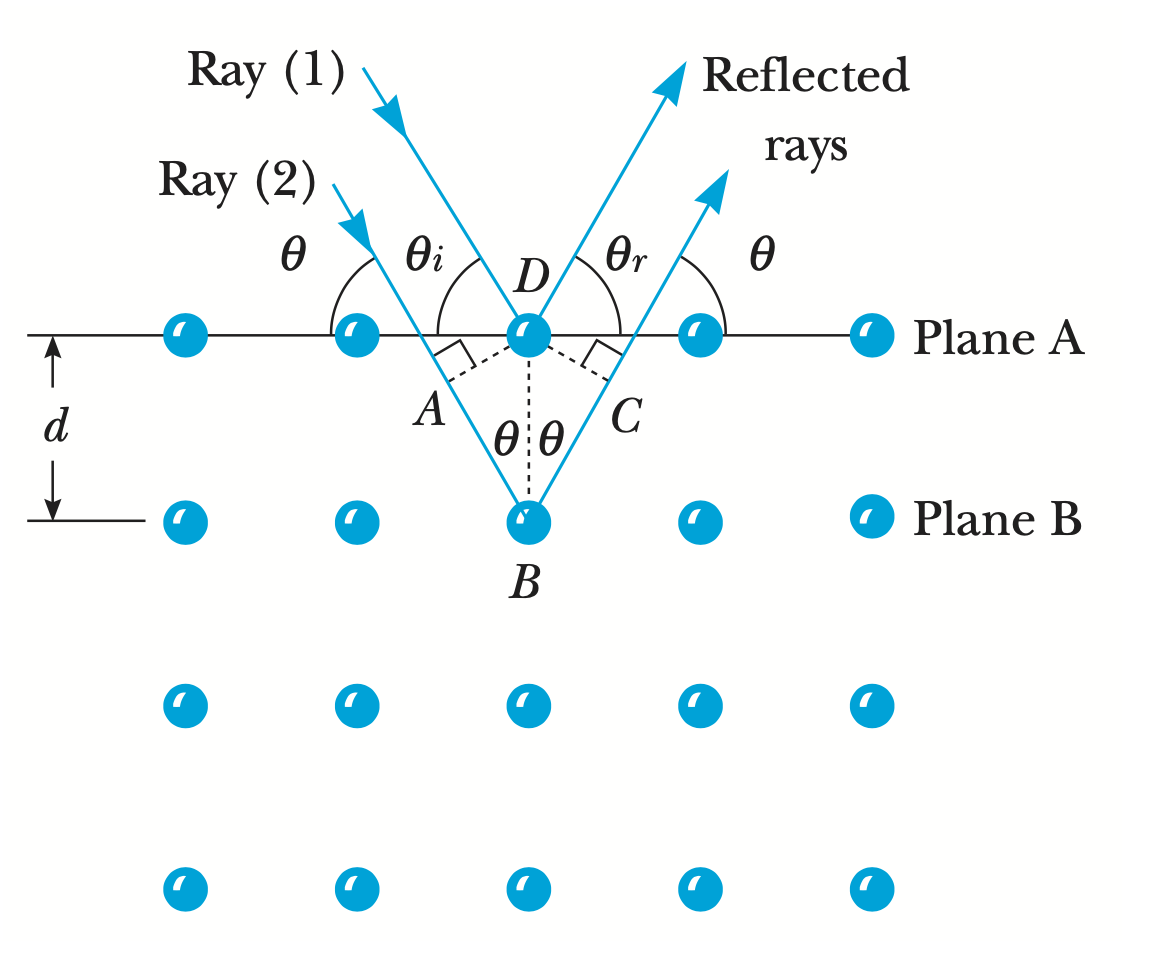
\includegraphics[width=0.9\linewidth]{figures/x-ray acattering.png}
        \caption{Bragg scattering of x-rays from successive planes of atoms.}
        \label{fig:Bragg scattering}
        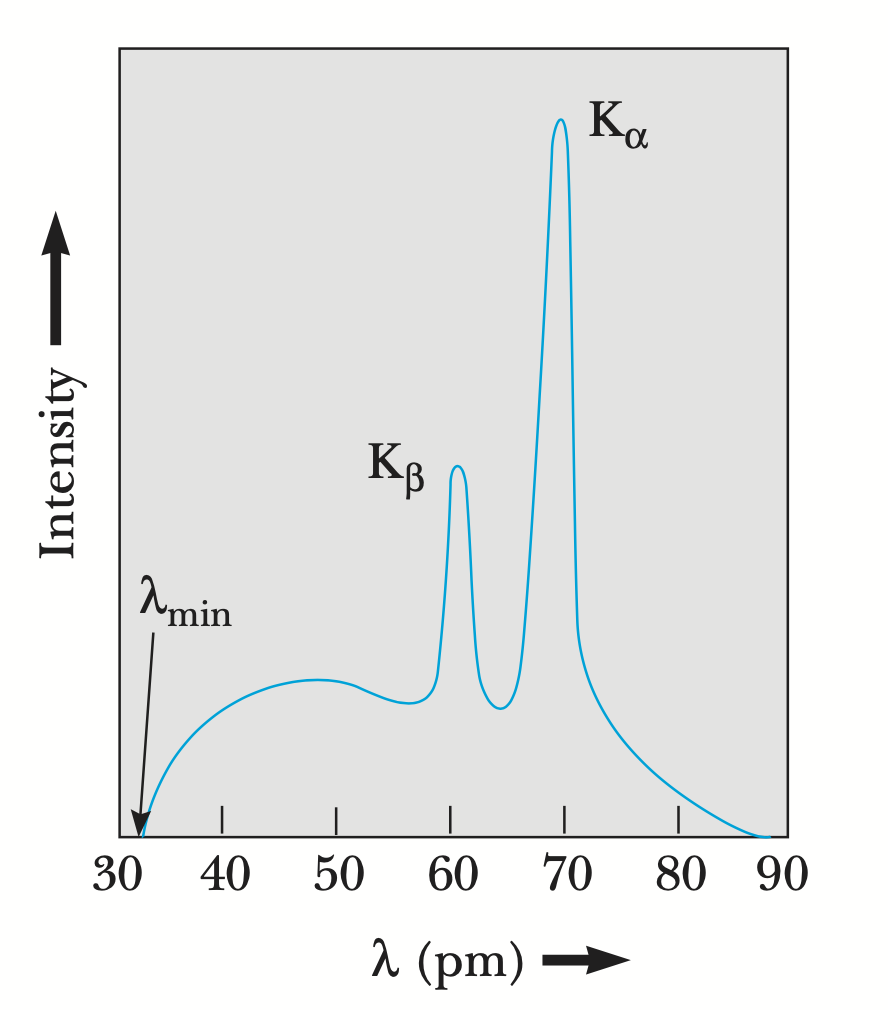
\includegraphics[width=0.9\linewidth]{figures/x-ray spectrum.png}
        \caption{The x-ray spectrum of a metal target.}
        \label{fig:x-ray spectrum}
    \end{wrapfigure}
    
    \paragraph{$\bullet$} A particularly simple method of analyzing the scattering of x-rays from parallel 
    crystal planes was proposed by W. L. Bragg in 1912. Consider two successive planes of atoms 
    as shown in Fig.\eqref{fig:Bragg scattering}.

    \paragraph{$\bullet$} The adjacent atoms in a single plane, $A$, will scatter constructively if the angle of 
    incidence, $\theta_i$, equals angel of reflaction, $\theta_r$.\\
    Atoms in \textit{successive planes} (A \& B), will scatter constructively if the the path length difference for rays (1) \& (2)
    is a ehole number of wavelength, thus $n\theta$, so 
    \begin{align}
        \label{The condition of scattering}
        \overline{AB} + \overline{BC} = n\theta, \qquad n=1, 2, 3, \dots
    \end{align}
    Thus Bragg equation is 
    \coloredeq{eq:Bragg equation}{\Delta{L} = 2d\sin{\theta} = n\lambda}
    {\tiny \begin{itemize}
        \item $n$ is the order of the intensity maximum, 
        \item $\lambda$ is the x-ray wavelength, 
        \item $d$ is the spacing between planes, 
        \item $\theta$ is the angle of the intensity maximum measured from plane $A$.
    \end{itemize}}
    If $\lambda$ is known $d$ of crystal can be found. If $d$ is also known, the x-ray intensity vs. wavelength may be determined
    as in Fig.\eqref{fig:x-ray spectrum}. This continuous x-ray spectrum results from glancing or indirect scattering 
    of electrons from metal atoms. In such collisions only part of the electron’s energy is converted to electromagnetic radiation.
    This radiation is called \textbf{bremsstrahlung} (German for braking radiation), which refers to the 
    radiation given off by any charged particle when it is \textit{decelerated}.

    \paragraph{$\bullet$} The $\lambda_{min}$ is independent of the target composition and only depends on the tube voltage, $V$.
    This might be explained by assuming it to the case of a \textit{head-on electron–atom collision} in which all of the 
    incident electron’s kinetic energy is converted to electromagnetic energy in the form of a single x-ray photon. For this case we have
    \begin{align}
        \label{eq:electron energy into x-ray}
        eV = hf = \frac{hc}{\lambda_{min}} \qquad or \quad \lambda_{min} = \frac{hc}{eV}
    \end{align}

    \begin{wrapfigure}{r}{0.3\linewidth}
        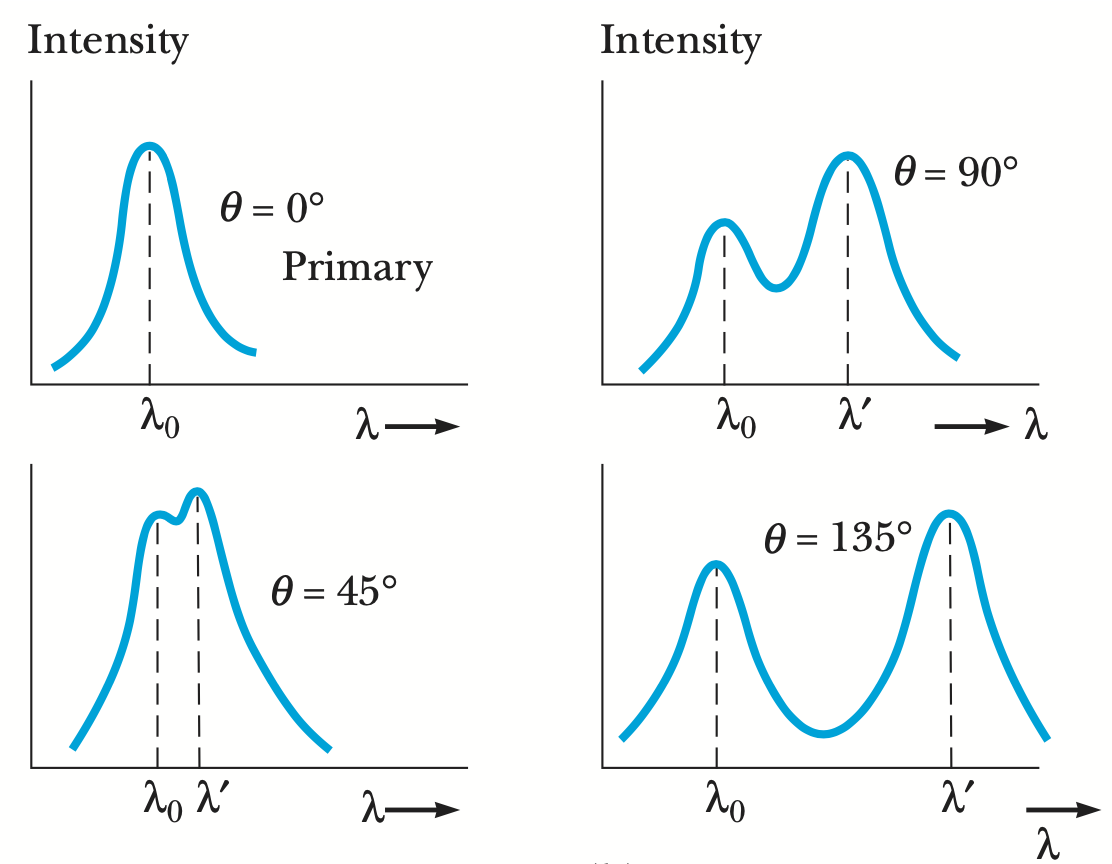
\includegraphics[width=0.9\linewidth]{figures/compton effect.png}
        \caption{Scattered x-ray intensity versus wavelength of Compton scattering.}
        \label{fig:Scattered x-ray}
        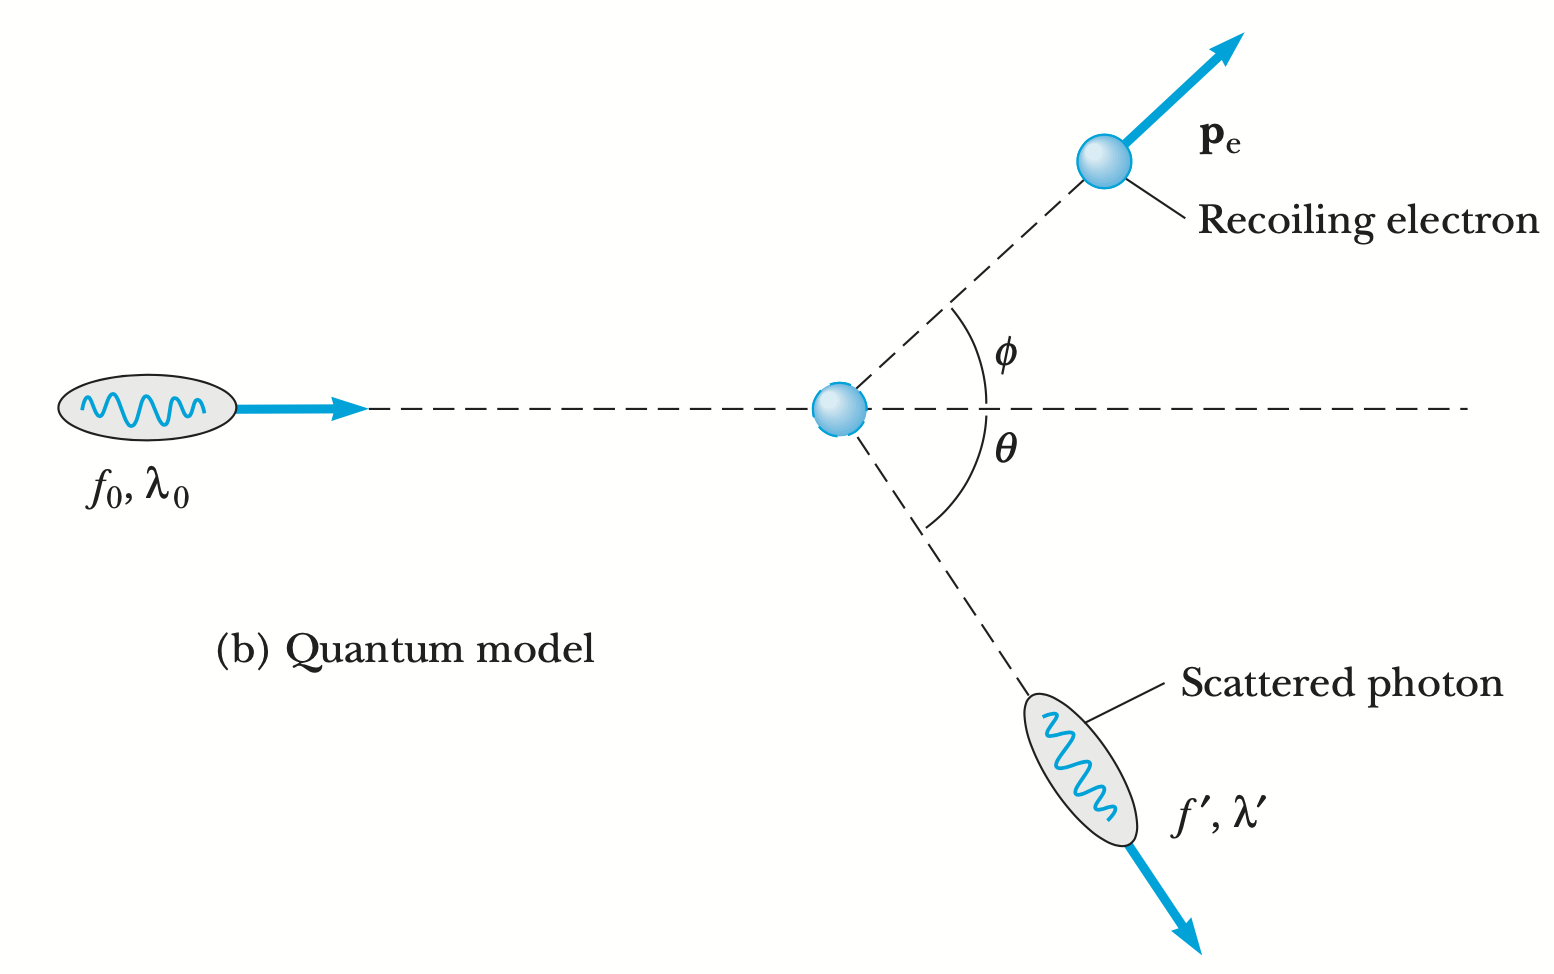
\includegraphics[width=0.9\linewidth]{figures/particle-like collision.png}
        \caption{The quantum view}
        \label{fig:scattered quantum x-ray}
    \end{wrapfigure}

    \paragraph{The Compton Effect} % (fold)
    \label{par:The Compton Effect}
    In 1922, Arthur Holly Compton confirmed that x-ray photons behave like particles with momentum $hf/c$.


    \paragraph{$\bullet$} classical theory predicted that incident radiation of frequency $f_0$ should accelerate an electron 
    in the direction of propagation of the incident radiation, and it should cause \textit{forced oscillations} of the electron 
    and reradiation at frequency $f'$, where $f' \le f$.\footnote{This decrease in frequency of the reradiated wave is caused 
    by a double Doppler shift, first because the electron is receding from the incident radiation, and second because the electron
    is a moving radiator as viewed from the fixed lab frame} The frequency or wavelength of the scattered radiation should depend 
    on the length of time the electron was exposed to the incident radiation as well as on the intensity of the incident radiation.

    \paragraph{$\bullet$} Compton's result was that the wavelength of the x-ray is independent of the intensity of radiation and
    exposure duration, and depends only on the scattering angle!.

    \paragraph{\color{c3}$\bigstar$} Quantum model easily explained the lower scattered frequency $f'$, where the incident photon gives 
    some its energy $hf$ and momentum to the recoiling electron.

    \paragraph{$\bullet$}  From Fig.\eqref{fig:Scattered x-ray} the shifted peak at $\lambda'$ is caused by the scattering of 
    x-rays from nearly free electrons. Assuming the photon exhibits particle-like behavior and collides elastically with a free
    electron initially at rest, Fig.\eqref{fig:scattered quantum x-ray}. Because electron recoils at high speed, we treat the
    collision relativistically. Thus from the energy conservation, 
    \begin{align}
        \label{eq:Compton derivation:1}
        E + m_ec^2 = E' + E_e
    \end{align}
    where $E$ is incident photon energy, $m_ec^2$ is the rest mass-energy of the electron, $E'$ is the energy of scattered
    photon, $E_e$ is the total relativistic energy of the electron after the collision. Likewise, by the momentum conservation, 
    \begin{align}
        \label{eq:Compton derivation:2}
        p  = p' \cos{\theta} + p_e \cos{\phi} &&
        p' \sin{\theta} = p_e \sin{\phi}
    \end{align}
    where $p$ is the momentum of the incident photon, $p'$ is the momentum of the scattered photon, and $p_e$ 
    is the recoiling electron momentum. We observed the angle of the scattered photons $\theta$, so we shall solve
    Eq.\eqref{eq:Compton derivation:1} and Eq.\eqref{eq:Compton derivation:2} simultaneously to eliminate $\phi$,
    \begin{align}
        \label{eq:Compton derivation:3}
        p_e^2 = p'^2 + p^2 - 2p p' \cos{\theta}
    \end{align}
    Paradoxically, we need to use the wave nature of light to explain the particle-like behavior 
    of photons. Recall that the energy of a photon and the frequency of the associated light wave are related 
    by $E=hf$. If we assume that a photon obeys the relativistic express $E^2 = p^2c^2 + m^2c c^4$, and the photon mass is zero, 
    \begin{align}
        \label{eq:Compton derivation:4}
        p_{photon} = \frac{E}{c} = \frac{hf}{c} = \frac{h}{\lambda}
    \end{align}
    A paradoxical situation; a particle property, the photon momentum, is given in terms of a wave property, $\lambda$, of 
    an associated light wave. If the relations $E = hf$ and $p = hf/c$ are substituted into 
    Eq.\eqref{eq:Compton derivation:1} and Eq.\eqref{eq:Compton derivation:3}, these become respectively
    \begin{align}
        \label{eq:Compton derivation:5}
        E_e = hf - hf' + m_e c^2, \qquad 
        p_e^2 = \left(\frac{hf'}{c}\right)^2 + \left(\frac{hf}{c}\right)^2 - \frac{2 h^2 f f' }{c2} \cos{\theta}
    \end{align}
    Because the Compton measurements do not concern the total energy and momentum of the electron, 
    we eliminate $E_e$ and $p_e$ by substituting Eq.\eqref{eq:Compton derivation:4} into the following expression for 
    the electron’s relativistic energy,
    \begin{align}
        \label{eq:C}
        E_e^2 = p_e^2c^2 + m_e^2 c^4
    \end{align}
    And we get the Compton's equation,
    \coloredeq{eq:Compton equation}{\lambda - \lambda' = \frac{h}{m_e c}(1-\cos{\theta})}
    {\tiny \begin{itemize}
        \item $\lambda_C = \frac{h}{m_e c}$ is Compton wavelength = \SI{0.0243}{\AA}
    \end{itemize}}
    % paragraph The Compton Effect (end)

    \paragraph{Particle-Wave Complementarity} % (fold)
    \label{par:Particle-Wave Complementarity}
    Compton effect offers evidence that when light \textit{interacts} with matter it behaves as if it were composed 
    of particles with energy $hf$ and momentum $h/\lambda$.
    % paragraph Particle-Wave Complementarity (end)